\include{preamble}
\usepackage{todonotes}
\usepackage{graphicx}
\usepackage{amssymb}
\title[More on Tree Models]{\LARGE More on Tree Models}
\subject{More on Tree Models}
\begin{document}

\begin{frame}
\titlepage
\end{frame}

\stretchon

\begin{frame}[fragile]{Option on Stock Paying a Continuous Dividend Yield}
    \begin{itemize}
\item For options paying continuous dividend yield at rate of $q$, 1 unit of the stock at time $T = 0$ becomes $e^{qT}$ units at time $T$.
\item Our portfolio replicating an option payoff that holds $\delta$ shares of the stock and $V(S_0, 0) - \delta S_0$ units of bond
worths  at time $T$
\begin{align*}
\underbrace{\delta S_T e^{qT}}_{\text{value of stock}} + \underbrace{e^{rT} (V_0 - \delta S_0)}_{\text{value of bond}}
\end{align*}
\end{itemize}
\end{frame}

\begin{frame}[fragile]
    \begin{itemize}
\item To replicate the option payoff $V$ at T, the equations to solve becomes
\begin{align} \begin{cases}
\delta S_u e^{qT} + e^{rT}(V_0 - \delta S_0) = V_u \\
\delta S_d e^{qT} + e^{rT}(V_0 - \delta S_0) = V_d \\
\end{cases}
\end{align}
The solution is
\begin{align} \begin{cases}
\delta = e^{-qT}\frac{V_u - V_d} {S_u - S_d} \\
V_0 = e^{-rT} \left( \underbrace{\frac{S_0e^{(r-q)T} - S_d}{S_u - S_d}}_{\text{risk neutral probabiliy}~~p} V_u + \underbrace{\frac{S_u-S_0e^{(r-q)T}}{S_u - S_d}}_{1 - p} V_d  \right)\\
\end{cases}
\end{align}
\end{itemize}
\end{frame}

\begin{frame}[fragile]
\begin{itemize}
\item Black-Scholes model for stock with continuous dividend rate:
\begin{align*}
\frac{dS_t}{S_t} = (r-q) dt + \sigma dW_t,~~~S_T = S_0 e^{(r-q-\frac12 \sigma^2)T + \sigma W_T}
\end{align*}
    \item Second moment to match
    \begin{align}
        \E[S_T^2] = e^{2(r-{\color{red}q})T + \sigma^2 T} = p u^2 + (1-p) d^2, ~~~ p = \frac{e^{r-q}T - d}{u-d}
\end{align}
\item CRR tree calibration (imposing $u = \frac1d$):
\begin{align}
& u = \frac{b + \sqrt{b^2 - 4}}{2} \\
& d = \frac{b - \sqrt{b^2 - 4}}{2} = \frac1u
\end{align} where $b = e^{(r-q)T+\sigma^{2}T} + e^{-(r-q)T}$

\end{itemize}
\end{frame}

\begin{frame}[fragile]{Option on Currencies}
    \begin{itemize}
        \item A foreign currency can be regarded as an asset providing
a yield at the foreign risk-free rate of interest, $r_f$.
        \item Therefore $p$ is set as
        \begin{align}
            p = \frac {e^{(r_d-r_f)t} - d}{u-d}
\end{align} where we normally use $r_d$ to represent domestic risk-free rate.
\item Pricing derivatives on stock with dividend, or foreign exchange rate --- just replace the growth rate of the asset by $r-q$
\item Note that future cash flow are still discounted by $r$
\end{itemize}
\end{frame}

\begin{frame}{Trees with Path Dependent Options}
\begin{itemize}
    \item We have priced path-dependent options, but only a small subset
    \item When we valuing the $i$-th time step for American Option and Barrier Knock-Out options, we are making assumptions about what happened until time step $t_i$
    \begin{itemize}
        \item the American option is not exercised at time steps prior to $t_i$
        \item the Barrier KO option has survived until time step $t_i$
    \end{itemize}
    \item In other words, our tree is pricing
    \begin{itemize}
        \item American option that is \textbf{not yet} exercised at each node
        \item Barrier option that is \textbf{not yet} knocked out at each node
    \end{itemize}
    \item How about other path-dependent options --- Knock-In option, Asian Option?
\end{itemize}
\end{frame}

\begin{frame}{Pricing Barrier Knock-In Options}
\begin{itemize}
    \item Knock-In options can be priced with KIKO parity:
    \begin{align*}
    \text{KO} + \text{KI} = \text{Underlying Payoff Value}
    \end{align*}
    --- if the barrier is triggered, you obtain the unederlying payoff from KO, otherwise you obtain the underlying payoff from KI.
    \item This is what we do in practice, to avoid arbitrage coming from numerical errors
    \item But what if there is no KIKO parity? How do we price KI's then?
    \pause
    \item We need to have two states at each tree node
    \begin{itemize}
    \item one node representing the barrier is not yet triggered
    \item one node representing the barrier has been triggered
    \end{itemize}
\end{itemize}
\end{frame}

\begin{frame}{Pricing Barrier Knock-In Options}
At time step $i$, for the $j$-th node $V_{i,j}$, we calculate two values
    \begin{itemize}
        \item $V_{i,j}[0]$: the value of the trade if up to $i-1$ step the barrier is not triggered
        \begin{align*}
            V_{i,j}[0] =
            \begin{cases}
                p V_{i+1, j}[0] + (1-p) V_{i+1, j+1}[0] ~~~\text{\scriptsize if $S_{i, j}$ does not hit the barrier}\\
                p V_{i+1, j}[1] + (1-p) V_{i+1, j+1}[1] ~~~\text{\scriptsize if $S_{i, j}$ hits the barrier}
            \end{cases}
        \end{align*}
        \item $V_{i,j}[1]$: the value of the trade if up to $i-1$ step the barrier is triggered
        \begin{align*}
            V_{i,j}[1] = p V_{i+1, j}[1] + (1-p) V_{i+1, j+1}[1]
        \end{align*}
        \item The value of the Knock-In option at time 0 is then $V_{0, 0}[0]$ if current stock price $S_0$ does not trigger the barrier, $V_{0, 0}[1]$ otherwise.
    \end{itemize}
\end{frame}

\begin{frame}[fragile]
We noticed that at each time step we are doing
\begin{align}
\vec{V}_{i, j} =
\begin{bmatrix}
V_{i, j}[0] \\
V_{i, j}[1]
\end{bmatrix} = f \left(
\begin{bmatrix}
\E_\probQ[V_{i_+, j}[0]] \\
\E_\probQ[V_{i_+, j}[1]]
\end{bmatrix}
\right) = f (\E_\probQ[\vec{V_{i_+, j}}])
\end{align}
That is
\begin{align*}
\vec{V}_{i, j} = f (\E_\probQ[\vec{V}_{i_+, j}])
\end{align*}
Same as our previous simple cases, except that now $\vec{V}$ is a vector, representing the continuation value of the trade under certain assumption.
\pause
\vfill
The function $f$ is the \verb+valueAtNode+ function in our implementation.
\end{frame}

\begin{frame}[fragile]{One minor step of Generalization to our Binomial Pricer}
Before extending our tree to deal with multiple states, we make a minor generalization to our \verb_binomialPricer_:
\begin{lstlisting}
def binomialPricer(S, r, vol, trade, n, calib):
    T = trade.expiry
    t = T / n
    (u, d, p) = calib(r, vol, t)
    # set up the last time slice, there are n+1 nodes at the last time slice
    # NOTE: instead of asking for payoff function, we ask for valueAtNode, and feed a None to continuation value to indicate that we are at terminal
    vs = [trade.valueAtNode(T, S*u**(n-i)*d**i, None) for i in range(n+1)]
    # iterate backward
    for i in range(n - 1, -1, -1):
        # calculate the value of each node at time slide i (i+1 nodes)
        for j in range(i + 1):
            nodeS = S * u ** (i - j) * d ** j
            continuation = math.exp(-r * t) * (vs[j] * p + vs[j + 1] * (1 - p))
            vs[j] = trade.valueAtNode(t * i, nodeS, continuation)
    return vs[0]
\end{lstlisting}
So our requirement to the \verb_trade_ now are: \verb_expiry_ and \verb_valueAtNode_.
\end{frame}

\begin{frame}[fragile]
On the tradeable side we extend \verb_valueAtNode_ to return \verb_payoff_ if \verb_continuation_ is \verb_None_
\begin{lstlisting}
class EuropeanOption():
    def __init__(self, expiry, strike, payoffType):
        self.expiry = expiry
        self.strike = strike
        self.payoffType = payoffType
    def payoff(self, S):
        if self.payoffType == PayoffType.Call:
            return max(S - self.strike, 0)
        elif self.payoffType == PayoffType.Put:
            return max(self.strike - S, 0)
        else:
            raise Exception("payoffType not supported: ", self.payoffType)

    def valueAtNode(self, t, S, continuation):
        # return payoff if we are at terminal slice
        if continuation == None:
            return self.payoff(S)
        else:
            return continuation
\end{lstlisting}
\end{frame}

\begin{frame}[fragile]{Binomial Tree Pricer for Multi-State Node Values}
\begin{itemize}
\item Now we can easily extend our \verb_binomialPricer_ to deal with multi-state node values
\item Just ask \verb_valueAtNode_ to take a \textbf{vector} of continuation values and returns a \textbf{vector} of node values
\begin{lstlisting}
def binomialPricerX(S, r, q, vol, trade, n, calib):
  T = trade.expiry
  t = T / n
  (u, d, p) = calib(r, q, vol, t)
  # set up the last time slice, n+1 nodes
  vs = [trade.valueAtNode(T, S*u**(n-i)*d**i, None) for i in range(n+1)]
  # we expect valueAtNode to return us a array of vector
  nStates = len(vs[0])  # getting the number of states for this trade
  for i in range(n - 1, -1, -1): # iterate backward
    # calculate the value of each node at time slide i
    for j in range(i + 1):
      nodeS, df = S*u**(i-j)*d**j, math.exp(-r*t)
      cont = [df*(vs[j][k]*p + vs[j+1][k]*(1-p)) for k in range(nStates)]
      vs[j] = trade.valueAtNode(t * i, nodeS, cont)
  return trade.valueAtNode(0, S, vs[0])
\end{lstlisting}
\item Definition and calculation of node values are delegated to tradeables.
\end{itemize}
\end{frame}

\begin{frame}[fragile]{Pricing Barrier Knock-In Option}
\begin{lstlisting}
class KnockInOption():
    def __init__(self, downBarrier, upBarrier, barrierStart, barrierEnd,...):
        ...
    def valueAtNode(self, t, S, continuation):
        if continuation == None:
            notKnockedInTerminalValue = 0
            if self.triggerBarrier(t, S):  # if the trade is not knocked in,
                # it is still possible to knock in at the last time step
                notKnockedInTerminalValue = self.underlyingOption.payoff(S)
            # if the trade is knocked in already
            knockedInTerminalValue = self.underlyingOption.payoff(S)
            return [notKnockedInTerminalValue, knockedInTerminalValue]
        else:
            nodeValues = continuation
            # calculate state 0: if no hit at previous steps
            if self.triggerBarrier(t, S):
                nodeValues[0] = continuation[1]
            # otherwise just carrier the two continuation values
        return nodeValues
\end{lstlisting}
Note how we segregate the general tree framework and tradeable specific pricing logic, like what we did for the simple one-state case.
\end{frame}

\begin{frame}[fragile]{Testing KIKO Parity}
\begin{lstlisting}
    opt = EuropeanOption(1, 105, PayoffType.Call)
    ki = KnockInOption(90, 120, 0, 1, opt)
    ko = KnockOutOption(90, 120, 0, 1, opt)
    S, r, vol = 100, 0.01, 0.2
    kiPrice = binomialPricerX(S, r, vol, ki, 300, crrCalib)
    koPrice = binomialPricer(S, r, vol, ko, 300, crrCalib)
    euroPrice = binomialPricer(S, r, vol, opt, 300, crrCalib)
    print("kiPrice = ", kiPrice)
    print("koPrice = ", koPrice)
    print("euroPrice = ", euroPrice)
    print("KIKO = ", kiPrice + koPrice)
\end{lstlisting}
\begin{verbatim}
    kiPrice =  6.001588670701864
    koPrice =  0.2944684814077655
    euroPrice =  6.296057152109632
    KIKO =  6.296057152109629
\end{verbatim}
\end{frame}

\begin{frame}[fragile]{Testing KIKO Parity}
\begin{lstlisting}[style=compactlst]
    kis = [binomialPricerX(S, r, vol, KnockInOption(90, 120, 0, 1, EuropeanOption(1, k, PayoffType.Call)), 300, crrCalib) for k in range(95, 115)]
    kos = [binomialPricer(S, r, vol, KnockOutOption(90, 120, 0, 1, EuropeanOption(1, k, PayoffType.Call)), 300, crrCalib) for k in range(95, 115)]
    euros = [binomialPricer(S, r, vol, EuropeanOption(1, k, PayoffType.Call), 300, crrCalib) for k in range(95, 115)]
    kikos = [abs(kis[i] + kos[i] - euros[i]) for i in range(len(kis))]
    plt.plot(range(95, 115), kikos, label="KI+KO-Euro")
    plt.legend(); plt.xlabel('strike'); plt.yscale('log')  # plot on log scale
    plt.savefig('../figs/kiko.eps', format='eps')
    plt.show()
\end{lstlisting}
\vspace{-3mm}
\begin{center}
\includegraphics[width=.6\textwidth]{figs/kiko.eps}
\end{center}
\end{frame}

\begin{frame}{Pricing Asian Options with Tree}
\begin{itemize}
\item Knock-In Option gives us an idea about how tree prices products that require knowledge of the past --- making assumptions about the past and calculate continuation values based on the assumptions
\item Pricing other path-dependent options with tree follow the same logic
\item Asian option: it looks at the average $\bar S$ of the stock prices observed on a given list of fixing dates $T_i, ~i \in [1, n]$. An Asian call option with strike K's payoff is:
\begin{align}
\max\left(\bar S - K, 0 \right)
\end{align}
\vspace{-3mm}
\begin{itemize}
\item Arithmetic average: $\bar S = \frac1n \sum_{i = 1}^n S_{T_i}$, more frequently seen, we illustrate using this variation
\item Geometric average: $\bar S = (\prod_{i = 1}^n S_{T_i})^{\frac1n}$, has analytic solution under Black-Scholes model
\end{itemize}
\item To value an Asian option on a tree node, what is the information about the past we need to know?  \pause The \textbf{accumulated average} up to the time of tree node $t$
\end{itemize}
\end{frame}

\begin{frame}[fragile]{Pricing Asian Option with Tree}
\begin{itemize}
\item Look at it from the last time step (last fixing date $T_n$): if we know $A = \frac1{n-1}\sum_{i=1}^{n-1}S_{T_i}$, the payoff becomes
\begin{align*}
& \max\left(\bar S - K, 0 \right) \\
& = \max\left(\frac1n((n-1)A + S_{T_n}) - K, 0 \right) \\
& = \frac1n \max(S_{T_n} - \underbrace{(nK - (n-1)A)}_{\bar K}, 0)
\end{align*}
It is just a function of $S_{T_n}$ if we know $A$.
\item So, we sample a list of $[A_1, A_2, \ldots, A_m]$, as the possible value of our auxiliary variable $A$, then we can value the product at a tree node \textbf{assuming} the accumulated average in the past is $A_i$.
\item Our \verb+valueAtNode+ function takes a vector of length $m$ \verb_continuationValues_ and returns a vector of length $m$ \verb_nodeValues_.
\end{itemize}
\end{frame}

\begin{frame}[fragile]{Pricing Asian Option with Tree}
\begin{itemize}
\item For the time steps between $n-1$ and $n$-th fixing date, node values are continuation values since $A$'s do not change.
\item At time step $k$ that falls on a fixing date $T_i$, the logic in \verb_valueAtNode_:
\begin{itemize}
\item We are aiming at calculating the value at node with stock price S, assuming the accumulated average is $A$, so the accumlated average after knowning $S$ is
\begin{align}
\hat A = (A \times i + S) / (i + 1)
\end{align}
\item Therefore, we need to calculate the continuation value for accumulated average $\hat A$.
\item We have the continuation value for a sampled list $[A_1, A_2, \ldots, A_m]$, $\hat A$ do not fall exactly on one of them, but we can interpolate
\begin{itemize}
\item Find the interval $j$ that $\hat A \in [A_{j}, A_{j+1}]$, the node value at $S$, assuming the accumulated average is $A$ is then
\begin{align*}
\frac{\hat A - A_j}{A_{j+1} - A_{j}} V_{j+1} + \frac{A_{j+1} - \hat A}{A_{j+1} - A_{j}} V_{j}
\end{align*}
\end{itemize}
\end{itemize}
\end{itemize}
\end{frame}

\begin{frame}[fragile]{Asian Option --- Implementation}
\begin{lstlisting}[style=compactlst]
class AsianOption():
    def __init__(self, fixings, payoffFun, As, nT):
        self.fixings = fixings
        self.payoffFun = payoffFun
        self.expiry = fixings[-1]
        self.nFix = len(fixings)
        self.As, self.nT, self.dt = As, nT, self.expiry / nT
    def onFixingDate(self, t):
        # we say t is on a fixing date if there is a fixing date in (t-dt, t]
        return filter(lambda x: x > t - self.dt and x<=t, self.fixings)
    def valueAtNode(self, t, S, continuation):
        if continuation == None:
            return [self.payoffFun((a*float(self.nFix-1) + S)/self.nFix) for a in self.As]
        else:
            nodeValues = continuation
            if self.onFixingDate(t):
                i = len(list(filter(lambda x: x < t, self.fixings))) # number of previous fixings
                if i > 0:
                    Ahats = [(a*(i-1) + S)/i for a in self.As]
                    nodeValues = [numpy.interp(a, self.As, continuation) for a in Ahats]
        return nodeValues
\end{lstlisting}
\scriptsize
We managed to price Asian option without changing our tree pricer again.
\vfill
Note that this implementation has a lot of room for improvements
\begin{itemize}
\item \verb_As_ and \verb_nT_ should not be part of \verb+__init__+
\item \verb_onFixingDate_ is called at each node, and it loops over all the fixing dates, it should be done only once
\end{itemize}
A better implementation would require a \verb_setup_ function and interaction with the tree's geometry
\end{frame}

\begin{frame}{Additive Binomial Tree}
It is also commonly seen that binomial trees use $X = \ln S$ as the state variable:
\begin{center}
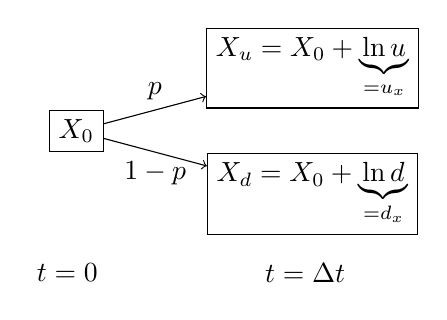
\begin{tikzpicture}
\tikzstyle{every node}=[draw,shape=rectangle];
\node (v0) at (-1, 0) {$X_0$};
\node (v1) at (2, 0.8) {$X_u = X_0 + \underbrace{\ln u}_{= u_x}$};
\node (v2) at (2, -0.8) {$X_d = X_0 + \underbrace{\ln d}_{= d_x}$};
\tikzstyle{every node}=[];
\draw [->] (v0) -- (v1) node[pos=.5,above] {$p$};
\draw [->] (v0) -- (v2) node[pos=.5,below] {$1-p$};
\node[text width=1cm] (t0) at (-1, -1.8) {$t=0$};
\node[text width=1.2cm] (t0) at (2, -1.8) {$t=\Delta t$};
\end{tikzpicture}
\end{center}
\end{frame}

\begin{frame}
\begin{center}
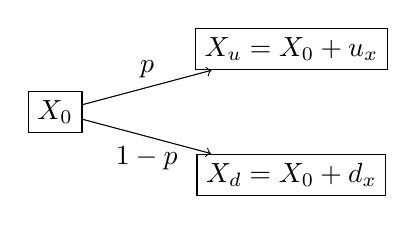
\begin{tikzpicture}
\tikzstyle{every node}=[draw,shape=rectangle];
\node (v0) at (-1, 0) {$X_0$};
\node (v1) at (2, 0.8) {$X_u = X_0 + u_x$};
\node (v2) at (2, -0.8) {$X_d = X_0 + d_x$};
\tikzstyle{every node}=[];
\draw [->] (v0) -- (v1) node[pos=.5,above] {$p$};
\draw [->] (v0) -- (v2) node[pos=.5,below] {$1-p$};
\end{tikzpicture}
\end{center}

The calibration formulas matching first and second moments of $X$ are:
\begin{itemize}
\item First moment
\begin{align}
\E[X] & = X_0 + p u_x + (1-p) d_x = \overbrace{X_0 + (r-\frac12 \sigma^2)\Delta t}^{\text{BS solution: } X = X_0 + (r - \frac12\sigma^2) \Delta t + \sigma W_{\Delta t}} \\
\Rightarrow ~~ & p u_x + (1-p) d_x = (r - \frac12 \sigma^2) \Delta t \\
\Rightarrow ~~ & p = \frac{(r - \frac12 \sigma^2) \Delta t - d_x}{u_x - d_x}
\label{eq:x_firstMoment}
\end{align}
\end{itemize}
\end{frame}

\begin{frame}
\begin{itemize}
\item Second moment
\begin{align}
\E[X^2] & = (X_0 + p u_x)^2 + (1-p) (X_0 + d_x)^2 \\
 & = X_0^2 + 2pX_0 u_x + 2(1-p)X_0d_x + pu_x^2 + (1-p)d_x^2 \\
 & = X_0^2 + 2X_0 \underbrace{(pu_x + (1-p)d_x)}_{(r-\frac12\sigma^2)\Delta t} + pu_x^2 + (1-p) d_x^2
\end{align}
Black-Scholes model's second moment:
\begin{align}
X_0^2 + 2X_0(r-\frac12 \sigma^2)\Delta t + (r-\frac12 \sigma^2)^2\Delta t^2 + \sigma^2 \underbrace{\E[W_{\Delta t}^2]}_{= \Delta t}
\end{align}
\item Equation for second moment:
\begin{align}
\label{eq:x_secondMoment}
pu_x^2 + (1-p)d_x^2 - (r-\frac12\sigma^2)^2 {\Delta t}^2 = \sigma^2 \Delta t
\end{align}
\end{itemize}
\end{frame}

\begin{frame}
\begin{itemize}
\item Knowning $p$ from \eqref{eq:x_firstMoment}, we have two unknowns $u_x$, $d_x$ and 1 equation \eqref{eq:x_secondMoment}.
\item Impose the constraint that $u_x = -d_x = \Delta x$, \eqref{eq:x_secondMoment} becomes
\begin{align}
\Delta x^2 & = \sigma^2 \Delta t + ((r-\frac12 \sigma^2)\Delta t)^2 \\
\Rightarrow \Delta x & = \sqrt{\sigma^2 \Delta t + ((r-\frac12 \sigma^2)\Delta t)^2} \\
             & \approx \sigma \sqrt{\Delta t}  ~~~\text{when}~~\Delta t \rightarrow 0
\end{align}
And
\begin{align}
p = \frac{(r - \frac12 \sigma^2) \Delta t - d_x}{u_x - d_x} = \frac12 + \frac{r- \sigma^2/2}{2 \sigma} \sqrt{\Delta t}
\end{align}
\item Pricing algorithm is the same as multiplicative trees, parameters can be demonstrated to be converging to each other
\item Bottom line --- when $\Delta t$ is small enough, all binomial model variations converges to Black-Scholes model
\end{itemize}
\end{frame}

\begin{frame}{Multi-dimensional Binomial Method}
\begin{block}{Spread Option}
A spread option gives the buyer the right to exchange a stock $S_2$ for $S_1$ at maturity $T$. Its payoff is $[S_1(T) - S_2(T)]_+$
\end{block}
\begin{itemize}
\item To price spread options whose payoff depends on two assets, we need two-dimensional binomial model
\item Assume both $S_1(t)$ and $S_2(t)$ follow Black-Scholes SDE
\begin{align}
& \frac{d S_1}{S_1} = (r-q_1) dt + \sigma_1 dW_1 \\
& \frac{d S_2}{S_2} = (r-q_2) dt + \sigma_2 dW_2 \\
& \rho dt = dW_1 dW_2
\end{align}
where $\rho$ is the correlation between the two assets, $q_1$ and $q_2$ are dividend rates of the two assets respectively.
\end{itemize}
\end{frame}

\begin{frame}{Multi-dimensional Binomial Model}
\begin{itemize}
\item Using additive tree, we have
\begin{align}
\begin{cases}
d x_1 = (r - q_1 - \frac12 \sigma_1^2) dt + \sigma_1 dt \\
d x_2 = (r - q_2 - \frac12 \sigma_2^2) dt + \sigma_2 dt
\end{cases}
\end{align}
\item Choosing equal up and down jump sizes $\Delta x_1$ and $\Delta x_2$, each tree step looks like:
\vspace{3mm}
\begin{center}
\includegraphics[width=.6\textwidth]{figs/twoDTree.png}
\end{center}
\end{itemize}
\end{frame}

\begin{frame}{Multi-dimensional Binomial Model - Calibration}
Denote $v_1 = r - q_1 - \frac12 \sigma_1^2$ and $v2 = r - q_2 - \frac12 \sigma_2^2$, to calibrate the model, we need to match the means, variances, and correlation:
\begin{align}
\begin{cases}
(p_{uu} + p_{ud}) \Delta x_1 - (p_{du} + p_{dd}) \Delta x_1 = v_1 \Delta t \\
(p_{uu} + p_{du}) \Delta x_2 - (p_{ud} + p_{dd}) \Delta x_2 = v_2 \Delta t \\
(p_{uu} + p_{ud}) \Delta x_1^2 + (p_{du} + p_{dd}) \Delta x_1^2 = \sigma_1^2 \Delta t + (v_1 \Delta t)^2 \approx \sigma_1^2 \Delta t \\
(p_{uu} + p_{du}) \Delta x_1^2 + (p_{ud} + p_{dd}) \Delta x_2^2 = \sigma_2^2 \Delta t + (v_2 \Delta t)^2 \approx \sigma_2^2 \Delta t \\
(p_{uu} - p_{ud} - p_{du} + p_{dd})\Delta x_1 \Delta x_2 = \rho \sigma_1 \sigma_2 \Delta t \\
p_{uu} + p_{ud} + p_{du} + p_{dd} = 1
\end{cases}
\end{align}
\end{frame}

\begin{frame}{Multi-dimensional Binomial Model - Calibration}
Solving the equation system, we have the model parameters:
\begin{align}
\begin{cases}
\Delta x_1 = \sigma_1 \sqrt{\Delta t} \\
\Delta x_2 = \sigma_2 \sqrt{\Delta t} \\
p_{uu} = \frac14 \frac{\Delta x_1 \Delta x_2 + \Delta x_2 v_1 \Delta t + \Delta x_1 v_2 \Delta t + \rho \sigma_1 \sigma_2 \Delta t}{\Delta x_1 \Delta x_2} \\
p_{ud} = \frac14 \frac{\Delta x_1 \Delta x_2 + \Delta x_2 v_1 \Delta t - \Delta x_1 v_2 \Delta t - \rho \sigma_1 \sigma_2 \Delta t}{\Delta x_1 \Delta x_2} \\
p_{du} = \frac14 \frac{\Delta x_1 \Delta x_2 - \Delta x_2 v_1 \Delta t + \Delta x_1 v_2 \Delta t - \rho \sigma_1 \sigma_2 \Delta t}{\Delta x_1 \Delta x_2} \\
p_{dd} = \frac14 \frac{\Delta x_1 \Delta x_2 - \Delta x_2 v_1 \Delta t - \Delta x_1 v_2 \Delta t + \rho \sigma_1 \sigma_2 \Delta t}{\Delta x_1 \Delta x_2}
\end{cases}
\end{align}
\end{frame}

\begin{frame}{Multi-dimensional Binomial Model}
\begin{itemize}
\item For every tree nodes (k, i, j), the assets' prices are calcualted by
\begin{align}
S_{1,k, i, j} = S_1 e^{(k - 2i) \Delta x_1}, ~~~S_{2, k, i, j} = S_2 e^{(k - 2j)\Delta x_2}
\end{align}
where $k$ denotes the time step, and $i, j$ represent the number of down movements for asset 1 and asset 2 from $t=0$.
\item At the end nodes of the tree, we calculate the payoff by
\begin{align}
max(0, S_1 - S_2)
\end{align}
\item The value at each node, $V(k, i, j)$ is given by:
\scriptsize
\begin{align}
V_{k, i, j} = e^{-r\Delta t} [p_{uu}V_{k+1, i, j} + p_{ud} V_{k+1, i, j+1} + p_{du} V_{k+1, i+1, j} + p_{dd} V_{k+1, i+1, j+1}]
\end{align}
\end{itemize}
\end{frame}

\begin{frame}{Analytic Solution for Spread Option --- Margrabe Formula}
\begin{itemize}
\item European style spread option can be priced analytically via a change of numeraire
\item If we price it using $S_2$ as numeraire, the option payoff would be $[\frac{S_1(T)}{S_2(T)} - 1]_+$ in unit of $S_2$ shares.
\item Under dollar measure, $\frac{S_1(T)}{S_2(T)}$'s volatility can be obtained using \Ito lemma
\begin{align*}
\sigma = \sqrt{\sigma_1^2 + \sigma_2^2 - 2\rho_{12}\sigma_1 \sigma_2}
\end{align*}
\item Changing measure to $S_2$ measure, the volatility does not change, and the risk-free interest rate becomes $S_2$'s dividend yield $q_2$
\item Now we have the diffusion of $\frac{S_1}{S_2}(t)$ under $S_2$ measure,
\begin{align}
d\left(\frac{S_1}{S_2}\right) = \frac{S_1}{S_2} ((q_2-q_1) dt + \sigma dW)
\end{align}
\end{itemize}
\end{frame}

\begin{frame}{Margrabe Formula: Change of Numeraire}
\begin{itemize}
\item The option can be priced with Black-Schole formula:
\begin{align}
e^{-q_1T} \frac{S_1(0)}{S_2(0)} N(d_1) - e^{-q_2T} N(d_2)
\end{align}
in unit of $S_2$, where
\begin{align}
& d_1 = \frac{\ln \frac{S_1(0)}{S_2(0)} + (q_2 - q_1 + \frac{\sigma^2}{2})T}{\sigma \sqrt{T}}
& d_2 = d_1 - \sigma\sqrt T
\end{align}
\item So converting it to dollar amount is merely a multiplication of $S_2(0)$:
\begin{align}
V_0 = e^{-q_1T} S_1(0) N(d_1) - e^{-q_2T} S_2(0) N(d_2)
\end{align}
\item We can use this formula to assess the accuracy of our two-dimensional tree.
\end{itemize}
\end{frame}


\begin{frame}{Trinomial Tree Model}
    \begin{itemize}
        \item Developed by Phelim Boyle in 1986
        \item An extension of binomial tree model
        \item The asset price can go up by a factor of $u$ or go down by a factor of $d$, or stay the same
with probability of $p_u$, $p_m$ and $p_d$ respectively
    \end{itemize}
\begin{center}
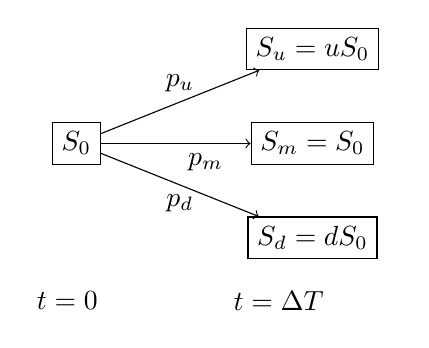
\begin{tikzpicture}
\tikzstyle{every node}=[draw,shape=rectangle];
\node (v0) at (-1, 0) {$S_0$};
\node (v1) at (2, 1.2) {$S_u = uS_0$};
\node (v2) at (2, 0.0) {$S_m = S_0$};
\node (v3) at (2, -1.2) {$S_d = dS_0$};
\tikzstyle{every node}=[];
\draw [->] (v0) -- (v1) node[pos=.5,above] {$p_u$};
\draw [->] (v0) -- (v2) node[pos=.7,below] {$p_m$};
\draw [->] (v0) -- (v3) node[pos=.5,below] {$p_d$};
\node[text width=1cm] (t0) at (-1, -2.) {$t=0$};
\node[text width=2cm] (t0) at (2, -2.) {$t=\Delta T$};
\end{tikzpicture}
\end{center}
\end{frame}

\begin{frame}
\begin{itemize}
\item To calibrate trinomial tree model parameters
\begin{align}
\begin{cases}
    e^{\mu \Delta t} = p_u u + p_m + p_d d  &~~~\rightarrow  \text{match first moment} \\
    e^{2\mu \Delta t + \sigma^2 t} = p_u u^2 + p_m + p_d d^2  &~~~\rightarrow \text{match second moment} \\
    u = \frac1d  &~~~\rightarrow \text{ensure nodes recombining} \\
    p_u + p_m + p_d = 1   ~~~~ &
\end{cases}
\end{align}
\item There are 5 unknows and 4 equations --- countless solution
\item Use $u = e^{\lambda \sigma \sqrt{\Delta t}}$, where $\lambda \geq 1 $ is a tunable parameter, then
    \begin{align}
        \begin{cases}
        p_u = \frac1{2\lambda^2} + \frac{\mu - \frac{\sigma^2}2}{2 \lambda \sigma} \sqrt{\Delta t} \\
        p_d = \frac1{2\lambda^2} - \frac{\mu - \frac{\sigma^2}2}{2 \lambda \sigma} \sqrt{\Delta t}
\end{cases}
    \end{align}
\end{itemize}
\end{frame}

\begin{frame}{Example}
\begin{itemize}
    \item Let $\lambda = \sqrt{3}$, we have
    \begin{align}
        \begin{cases}
u = e^{\sqrt{3 \Delta t}}, ~~~ d = e^{-\sqrt{3 \Delta t}} \\
p_u = \frac16 + \frac{\mu - \frac{\sigma^2}2}{\sqrt{12} \sigma} \sqrt{\Delta t} \\
p_d = \frac16 - \frac{\mu - \frac{\sigma^2}2}{\sqrt{12} \sigma} \sqrt{\Delta t} \\
p_m = \frac23
\end{cases}
\end{align}
\end{itemize}
\end{frame}

\begin{frame}[fragile]{Trinomial Tree Implementation}
\begin{lstlisting}
def trinomialPricer(S, r, q, vol, trade, n, lmda):
    t = trade.expiry / n
    u = math.exp(lmda * vol * math.sqrt(t))
    mu = r - q
    stdev = vol*math.sqrt(t)
    pu = 0.5/lmda/lmda + (mu-vol*vol/2)/2/lmda/stdev
    pd = 0.5/lmda/lmda - (mu-vol*vol/2)/2/lmda/stdev
    pm = 1 - pu - pd
    # set up the last time slice, there are 2n+1 nodes at the last time slice
    # counting from the top, the i-th node's stock price is S * u^(n - i),
    # i from 0 to n+1
    vs = [trade.payoff(S * u ** (n - i)) for i in range(2*n + 1)]
    # iterate backward
    for i in range(n - 1, -1, -1):
        # calculate the value of each node at time slide i, there are i nodes
        for j in range(2*i + 1):
            nodeS = S * u ** (i - j)
            continuation = math.exp(-r*t)*(vs[j]*pu + vs[j+1]*pm + vs[j+2]*pd)
            vs[j] = trade.valueAtNode(t * i, nodeS, continuation)
    return vs[0]
\end{lstlisting}
\end{frame}

\begin{frame}[fragile]{Trinomial Tree vs Binomial Tree}
\begin{lstlisting}[style=compactlst]
    opt = EuropeanOption(1, 105, PayoffType.Call)
    S, r, vol, n = 100, 0.01, 0.2, 300
    bsprc = bsPrice(S, r, vol, opt.expiry, opt.strike, opt.payoffType)
    crrErrs = [math.log(abs(binomialPricer(S, r, vol, opt, i, crrCalib) - bsprc)) for i in range(1, n)]
    jrrnErrs = [math.log(abs(binomialPricer(S, r, vol, opt, i, jrrnCalib) - bsprc)) for i in range(1, n)]
    jreqErrs = [math.log(abs(binomialPricer(S, r, vol, opt, i, jreqCalib) - bsprc)) for i in range(1, n)]
    tianErrs = [math.log(abs(binomialPricer(S, r, vol, opt, i, tianCalib) - bsprc)) for i in range(1, n)]
    plt.plot(range(1, n), crrErrs, label = "crr")
    plt.plot(range(1, n), jrrnErrs, label = "jrrn")
    plt.plot(range(1, n), jreqErrs, label = "jreq")
    plt.plot(range(1, n), tianErrs, label="tian"), plt.legend()
    plt.savefig('../figs/triError.eps', format='eps')
\end{lstlisting}
\vspace{-4mm}
\begin{center}
\includegraphics[width=0.5\textwidth]{figs/triError.eps}
\end{center}
\end{frame}

\begin{frame}{Trinomial Tree vs Binomial Tree}
\begin{itemize}
\item Trinomial tree is considered to produce more accurate results than binomial tree (marginal in my opinion)
\item The extra node and parameter gives some freedom to position tree nodes at critical points of the payoff, for example
\begin{itemize}
\item Discontinuity point at payoff
\item Barrier level, and with the center state, trinomial tree allows having node at barrier value at each time step
\end{itemize}
\end{itemize}
\end{frame}

\end{document}
\begin{frame}
    multi-dimensional binomial tree  --- summarize
    example
    greeks stability - similar
    comparison between binomial and trinomial
    computation cost
\end{frame}


\begin{frame}
    Binomial tree and Greeks

Greeks measure the sensitivity of the price of derivatives such as options to a
change in underlying asset’s parameters. They are used for hedging and risk
management.
Delta: measures the rate of change of the theoretical option value with
respect to changes in the underlying asset's price.
It is the first derivative of the option value C with respect to the
underlying instrument’s price S.
   C
 S
   C
 r
Theta: the rate of change in the price of an option with respect to time.    C
 T
Vega: the rate of change in the price of an option to a unit change in
volatility, σ.    C
 
Pho: the rate of change in the price of an option in response to a
change in the interest rate.
Gamma: the rate of change in the delta to the price, S
 2 C  
  2 
 S
 S
\end{frame}


\begin{frame}
    Time vary volatility, implied tree

Time varying volatility is used in practice.
Implied volatility is obtained from the market price of the options.
The option price should be consistent with these observed
volatilities.
In a trinomial tree, for time step i, we have time varying volatility  i
and time varying probabilities p i the parameter u and d satisfy
the following equations
p i S 0 u  ( 1  p i ) S 0 d  S 0 e rdt
p i ( u ) 2  ( 1  p i )( d ) 2  [ p i u  ( 1  p i ) d ] 2   i dt
\end{frame}


%
%the expectation of the stock price under risk neutral measure is
%\begin{align}
%    F = E_\probQ[S_T] = S_0 e^{(r-q)T}
%\end{align}
%Why so? Because
%The total



%
%Therefore,
%\begin{align}
%    p = \frac{e^{(r-q)T} - d}{u - d}
%\end{align}
%why so?



%\begin{frame}[fragile]{Another way to calibrate CRR Binomial Tree}
%Recall that to match the second moment we need to solve $u, v$ such that
%\begin{align}
%    e^{2\mu t + \sigma^2 t} = p u^2 + (1-p) d^2
%\end{align}
%Expand the LHS using Taylor:
%\begin{align}
%    e^{2\mu t + \sigma^2 t} \approx 1 + (2\mu t + \sigma^2 t)
%\end{align}
%   derive approximation $u = e^{\sigma \sqrt{t}}$
%\end{frame}
%\end{document}

